\chapter{Lenguaje P4}
%%%%%%%%%%%%%%%%%%%%%%%%%%%%% Info útil  %%%%%%%%%%%%%%%%%%%%%%%%%%%%%
\section{Enlaces útiles}
\begin{itemize}
    \item Tutoriales: \url{https://github.com/p4lang/tutorials/}
    \item Protobuf: \url{https://developers.google.com/protocol-buffers/}
    \item gRPC: \url{https://grpc.io/}
    \item gRPC ejemplo: \url{https://www.nocountryforgeeks.com/grpc-protocol-buffers/}
    \item Lista de reproducción sobre conferencias: \newline 
    \url{https://www.youtube.com/playlist?list=PLRffjASqEa5VMsUml2V34_xDTeVydeM_L}
    \item Correo explicando BM2: \url{http://lists.p4.org/pipermail/p4-dev_lists.p4.org/2016-June/002112.html}
    
\end{itemize}
\section{Papers de interés}
\begin{itemize}
    \item Paper sobre la agregación de tecnología p4 para parsear paquetes generados por sensores IoT a una WAN \cite{p4_iot-paper}.
    \item Paper sobre como emplear Switches p4 frontera para servicios de IoT \cite{8470257}
    \item Paper sobre el gran potencial que tiene p4 para interconectar el mundo SDN con la próxima generación de nodos finales que interactúan con clusters de TI innovadores, 5G fronthaul e internet de las cosas. \cite{8651200}
    
\end{itemize}
%%%%%%%%%%%%%%%%%%%%%%%%%%%%% Intro Teórica %%%%%%%%%%%%%%%%%%%%%%%%%%%%%

\section{Introducción teórica}
En este punto se va a tratar de abordar todos los conceptos teóricos que nos vayan surgiendo según exploramos p4. Se intentará tratar de entender todas las tecnologías que emplea p4, cual es su uso, cuales son sus pros y sus posibles contras. 
\subsection{¿Qué es P4?}
{}

\newpage
%%%%%%%%%%%%%%%%%%%%%%%%%%%%% Instalación %%%%%%%%%%%%%%%%%%%%%%%%%%%%%
\section{Instalación}
\begin{itemize}
    \item Hemos instalado una máquina virtual de Ubuntu 16.04, con 20GB de almacenamiento ya que con 10 se nos queda corto. 4 GiB de ram y cuatro núcleos
    
    \item Hemos hecho un update y upgrade, e instalado git, vim, htop, openssh-server para conectarse vía ssh en remoto.
    
    \item Hemos hecho un git clone del repositorio con el tutorial:
    \url{https://github.com/p4lang/tutorials}
    
    \item Lanzamos los dos shell-scripts user-bootstrap.sh y root-bootstrap.sh. 
    \item Hemos encontrado varios problemas en el momento de llevar a cabo la instalación. Por lo que se ha decidido modificar los shells-scripts de instalación ofrecidos en el repositorio.
\end{itemize}

Como se ha introducido antes, hemos tenido que crear nuestro propio script de instalación \textbf{install.sh}. Habrá que darle permisos de ejecución \textbf{chmod 777 install.sh} y lanzarlo con \textbf{sudo}. \newline
\newline

La necesidad de crear otro método de instalación es la deficiencia del los métodos alternativos de instalación que tienen aparte de Vagrant. Ellos disponen de dos shell-scripts, donde crean un enviroment muy cercano a personas con poco conocimiento de Linux, facilitándoles user propio p4, generar iconos en el escritorio, configurar IDEs... Tareas propias de cada de desarrollador en función de sus preferencias. \newline
\newline

Por lo que se ha decidido limpiar el proceso de instalación, dejando únicamente lo estrictamente necesario para llevar a cabo el tutorial de p4. Dejando únicamente un shell-script, más optimizado y  más limpio. Se ha tenido que hacer una doble llamada al shell-script \textbf{autogen.sh} debido a este issue:  
\begin{itemize}
    \item \url{https://github.com/protocolbuffers/protobuf/issues/149} 
\end{itemize}
Como forma de agradecer a la organización de p4 el hecho de que tengan un buen repositorio de tutoriales dando un buen entrypoint para los noobies que acaban de empezar con p4 (Yo) se ha ofrecido el script de instalación para que se incorpore al master.\newline
\newline
Al hacer el pull-request, el mantenedor de los tutoriales le pareció una buena idea, pero el hecho de tener un método de instalación nuevo significa más trabajo para mantener el repositorio. Me pidió que tratara de incluir la instalación nativa de Vagrant para que así con un único script podamos tener la instalación sobre Vagrant y el método que habíamos propuesto. Para poder llevar esta tarea a cabo se tuvo que estudiar la herramienta de Vagrant. En los anexos se han puesto unas pinceladas de los aspectos más significativos de esta herramienta. \newline
\newline
De momento no está incluido en el master pero se puede hacer de uso del nuevo método de instalación el fork creado de los tutoriales de p4.
\begin{itemize}
    \item \url{https://github.com/davidcawork/testP4/tree/master/tutorial}
\end{itemize}
Se puede consultar el estado del pull-request aquí.
\begin{itemize}
    \item \url{https://github.com/p4lang/tutorials/pull/261}
\end{itemize}

Para llevar a cabo la instalación del modo nativo sobre Vagrant se debe instalar Vagrant, instalar un proveedor de maquinas virtuales y cargar el VagrantFile. Para más información sobre el uso de Vagrant consulte la información referente a ello en los anexos.
\newpage
%%%%%%%%%%%%%%%%%%%%%%%%%%%%% Tutoriales %%%%%%%%%%%%%%%%%%%%%%%%%%%%%
\section{Test P4}
En esta sección vamos a seguir el tutorial y los test que proponen la organización de p4 en su repositorio oficial.
\begin{itemize}
    \item \url{https://github.com/p4lang/tutorials}
\end{itemize}
La metodología de los tutoriales consiste en completar el esqueleto del código p4 dado por ellos para hacer funcionar las distintas pruebas. El escenario que se ha empleado para establecer un eviroment de pruebas es Mininet.

\section{Test 1: Implementando el fordwarding básico}

El objetivo de este test es escribir un programa P4 que implemente el fordwarding básico. Con el reenvío de IPv4, el conmutador debe realizar las siguientes acciones para cada paquete:
\begin{itemize}
    \item Actualizar las direcciones MAC de origen y destino.
    \item Disminuir el campo de la cabecera IP (TTL).
    \item Reenviar el empaquete el puerto apropiado.
\end{itemize}

Nuestro router tendrá una sola tabla, que el plano de control llenará con reglas estáticas. Cada regla asignará una dirección IP a la dirección MAC y al puerto de salida para el próximo salto. Ya se han definido las reglas del plano de control, por lo que solo necesitamos implementar la lógica del plano de datos de nuestro programa P4 (\textit{basic.p4}).

\subsection{Comprobar el modelo suministrado}
En este punto siguiendo el tutorial, tenemos que comprobar como efectivamente el modelo suministrado no es capaz de establecer comunicaciones entre nodos finales. Esto se debe a que el plano de datos de los routers está incompleto, y será nuestra misión la de completar el plano de datos con nuestro programa en p4 que dotará de la capacidad de fordwarding de paquetes a los routers. \newline
\newline
Procedimiento a seguir para llevar a cabo el test:
\begin{itemize}
    \item Hacemos uso del Makefile que trae el tutorial: \textbf{make run}, este target del Makefile automatizará las siguientes tareas:
    \begin{itemize}
        \item Compilará el archivo \textit{basic.p4} para el behavioral model 2 (bm2) el target simple switch
        \item Lanzará Mininet con una topología de tres router conectados triangularmente y a cada router se conectará un host. Los host tendrán respectivamente las IPs 10.0.1.1, 10.0.2.2, 10.0.3.3. 
    \end{itemize}
    \item En el mismo directorio se encuentran dos herramientas escritas en Python, servidor y cliente, que nos ayudaran a generar tráfico desde un host a otro. Estas herramientas hacen uso de Scapy para poder visualizar el contenido el paquete generado. Herramientas \textit{receive.py} y \textit{send.py}. 
    \item Levantaremos dos terminales por ejemplo, host 1 y host 2: \textbf{xterm h1 h2}
    \item Ejecutaremos las herramientas para generar tráfico entre ambos host.
    \item El mensaje no llegará, salimos de Mininet con \textbf{exit}, y limpiamos el escenario y Mininet con \textbf{make stop} (Este target llamará a \textbf{sudo mn -c} por nosotros).
\end{itemize}

%%%%%%%%%%%%%%%%%%%%%%%% foto terminales %%%%%%%%%%%%%%%%%%%%%%%%%

\begin{figure}[!htb]
  \centering
    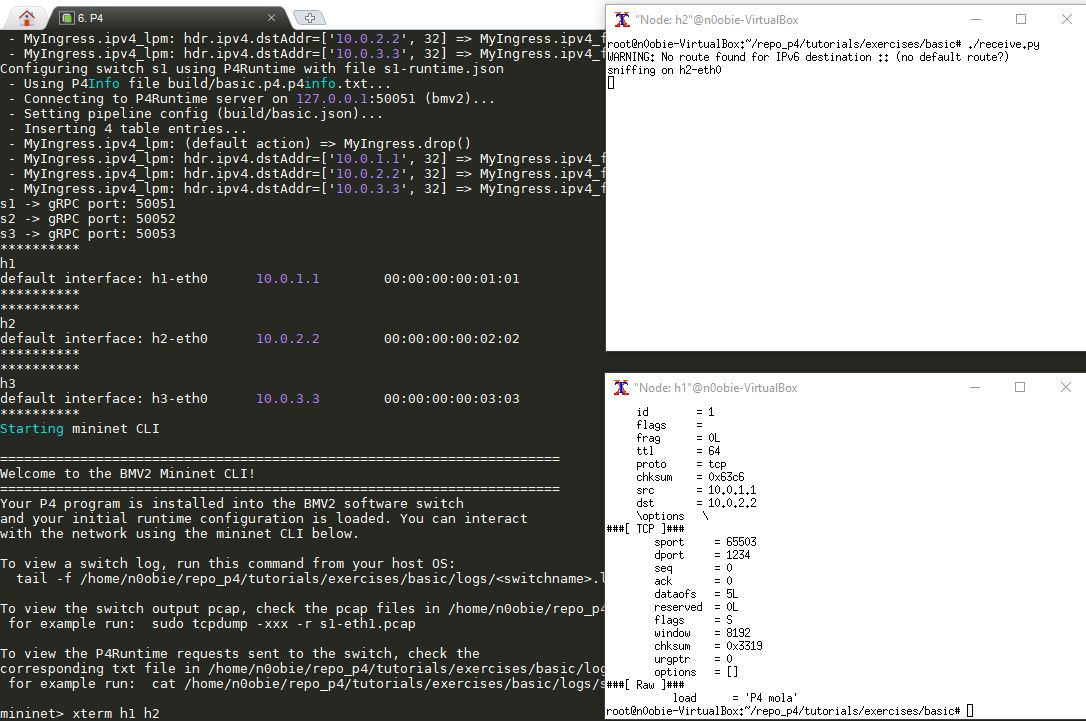
\includegraphics[width=\linewidth]{./img/test/1.JPG}
    \caption{Test Mininet: No llega el mensaje.}
  \label{fig:yo}
\end{figure}

%%%%%%%%%%%%%%%%%%%%%%%% foto terminales %%%%%%%%%%%%%%%%%%%%%%%%%

Un programa P4 define una pipe-line de procesamiento de paquetes, pero las reglas dentro de cada tabla se insertan desde el plano de control. Cuando una regla coincide con un paquete (Hay un hit), su acción se invoca con los parámetros proporcionados por el plano de control como parte de la regla.\newline
\newline
En este test, ya se ha implementado la lógica del plano de control, está suministrado por el equipo de p4. A la hora de levantar la instancia de Mininet, el comando make run instalará las reglas de procesamiento de paquetes en las tablas de cada router. Estas se definen en los archivos sX-runtime.json, donde X corresponde al número de router.\newline
\newline
Se hace uso de P4Runtime para instalar las reglas del plano de control. El contenido de los archivos sX-runtime.json se refiere a nombres específicos de tablas, claves y acciones, tal como se define en el archivo P4Info producido por el compilador (busque el archivo build / basic.p4info después de ejecutar make run). Cualquier cambio en el programa P4 que agregue o cambie el nombre de tablas, claves o acciones deberá reflejarse en estos archivos sX-runtime.json.

\subsection{Desarrollo del fordwarding L3}
El archivo basic.p4 contiene un programa P4 esqueleto con piezas lógicas clave donde deberemos completar su cuerpo para el correcto funcionamiento del router. Las partes que debemos completar son las siguientes:
\begin{itemize}
    \item Completar el Parser para extraer las cabeceras de ethernet e ipv4.
    \item Completar un action llamado forward\_ipv4 que deberá: 
        \begin{itemize}
            \item Establecer el puerto de salida del paquete. 
            \item Establecer como dirección MAC origen la MAC destino de la trama recibida. 
            \item Establecer como dirección MAC destino del paquete la MAC del siguiente salto.
            \item Decrementar el campo TTL de la cabecera ipv4.
        \end{itemize}
    
    \item Completar el campo apply para decidir si aplicar la tabla.
\end{itemize}
\newpage
Para completar el parser de entrada del router hemos definido tres estados, el primer estado, entry-point, llamado start. El segundo parse\_ethernet, para extraer la cabecera de Ethernet, y decidir si si entramos a la ultima fase del parser, parse\_ipv4, en función del campo etherType. La ultima fase del parser únicamente extrae la cabecera de Ipv4. 
\begin{figure}[!htb]
  \centering
    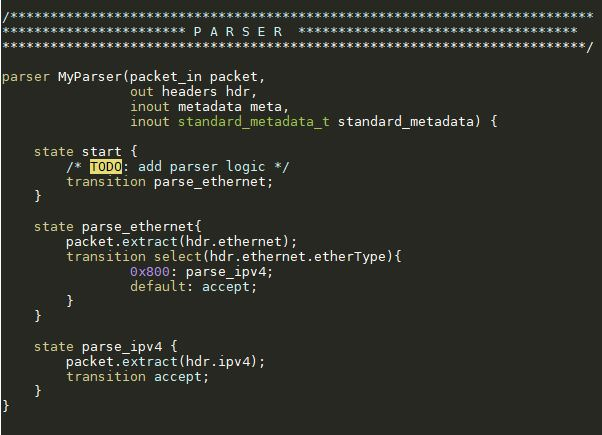
\includegraphics[width=0.8\linewidth]{./img/test/2.JPG}
    \caption{Parser.}
  \label{fig:yo}
\end{figure}
\newline
Hemos definido un action que hacer forwarding a los paquetes que les llega a los router, deberá especificar un puerto de salida, modificar las MAC para el siguiente hop, y decrementar en uno el campo TTL de la cabecera Ipv4. \newline

\begin{figure}[!htb]
  \centering
    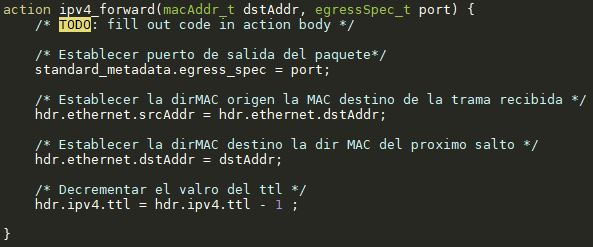
\includegraphics[width=0.8\linewidth]{./img/test/3.JPG}
    \caption{Action forwarding.}
  \label{fig:yo}
\end{figure}
Según los requerimientos dados, debemos comprobar con anterioridad si existe y es valida la cabecera Ipv4.
\newpage
\begin{figure}[!htb]
  \centering
    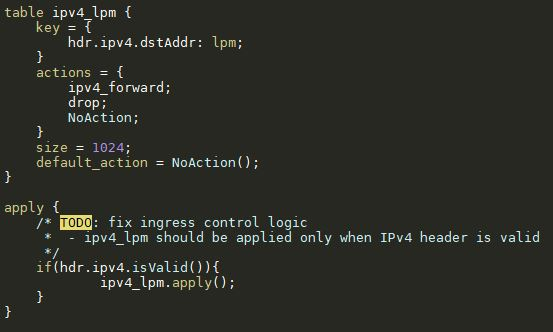
\includegraphics[width=0.7\linewidth]{./img/test/4.JPG}
    \caption{Tabla match-action de nuestro router.}
  \label{fig:yo}
\end{figure}
Por último, únicamente debemos especificar en el deparser como queremos serializar las cabeceras, y en que orden. A continuación, se incluirá la carga útil y se conformará el paquete. Por carga útil entendemos toda información no procesada por el parser de entrada por el switch p4.
\begin{figure}[!htb]
  \centering
    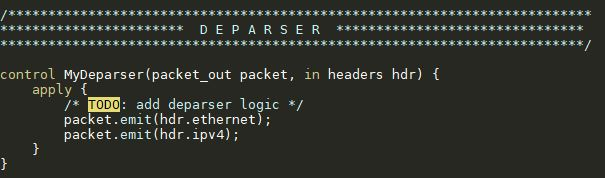
\includegraphics[width=0.8\linewidth]{./img/test/5.JPG}
    \caption{Deparser de nuestro router.}
  \label{fig:yo}
\end{figure}
\newline
\newline
A continuación, se puede apreciar en la arquitectura conformada en bloques de nuestro switch. Donde, cada bloque va especificando la funcionalidad para la que ha sido programada. Este diseño es muy útil para ver de manera la operativa funcional de nuestro switch.
\newline
\newline
\begin{figure}[!htb]
  \centering
    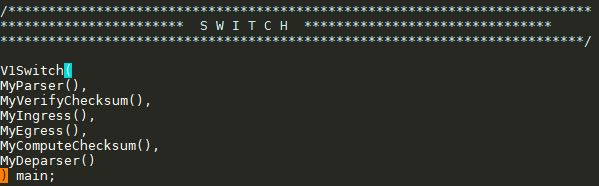
\includegraphics[width=0.8\linewidth]{./img/test/6.JPG}
    \caption{Topología funcional de nuestro switch.}
  \label{fig:yo}
\end{figure}
\newpage
A continuación, se expone como tras implementar los cambios existe conectividad en la topología entre todos los host. Para implementar los cambios antes hemos realizado un \textbf{sudo make stop} y un \textbf{sudo make clean} para limpiar los archivos residuales de los switch p4 y de Mininet.
\begin{figure}[!htb]
  \centering
    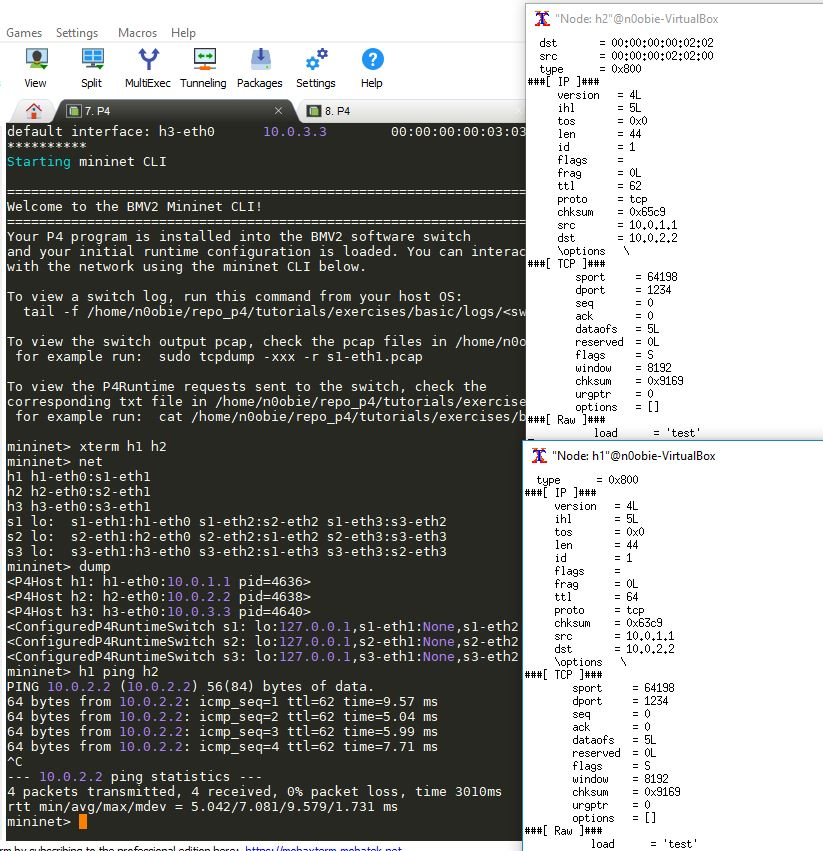
\includegraphics[width=\linewidth]{./img/test/7.JPG}
    \caption{Funcionamiento de router programado.}
  \label{fig:yo}
\end{figure}
\newpage
%%%%%%%%%%%%%%%%%%%%%%%%%%%%%%%%%%%%%%%%%%%%%%%%%%%%%%%%%%%%%%%%%%%%%%%%%%%%%%%%%%%%%%%%%%%%%%%%%%%%%%%%%%%%%%%%%%%%%%%%%%%%%%%%%%
\section{Test 2: Implementando el tunelado básico}

En este test, agregaremos soporte para un protocolo de tunelado básico al router que hicimos en el test anterior. El router básico reenvía en función de la dirección IP de destino. Tendremos que definir un nuevo tipo de encabezado para encapsular el paquete IP y modificar el código del router, para que en su lugar decida el puerto de salida utilizando una nueva cabecera de túnel.\newline
\newline
El nuevo tipo de cabecera contendrá una ID de protocolo, que indica el tipo de paquete que se está encapsulando, junto con una ID de destino que se utilizará para el enrutamiento.

\subsection{Crear protocolo de tunelado}
Siguiendo la guía debemos completar los siguientes items para conseguir el resultado del tunel entre los host.
\begin{itemize}
    \item Se debe actualizar el parser para extraer la cabecera de  myTunnel o la cabecera de  ipv4 según el campo etherType en la cabecera de  Ethernet. El etherType correspondiente al encabezado \textbf{myTunnel es 0x1212}. El parser también debe extraer el encabezado ipv4 después del encabezado myTunnel si proto\_id == TYPE\_IPV4.
    
    \item  Debemos definir una nueva acción llamada \textbf{myTunnel\_forward} que deberá situar el puerto de salida dado por el plano de control.
    
    \item Definir una tabla llamada como \textbf{myTunnel\_exact}. Esta tabla se encargará de asociar de forma exacta dado un dst\_id e invocará la acción programada anteriormente para especificar un puerto de salida idoneo para el dst\_id dado. Por defecto hará un drop.
    
    \item Hay que modificar el campo de \textbf{apply} del bloque de control de \textbf{MyIngress}. Este deberá aplicar en un primer caso la tabla \textbf{myTunnel\_exact} siempre y cuando se encuentre la cabecera myTunnel. En caso contrario se deberá aplicar la tabla del test anterior de ipv4\_lpm.
    
    \item Hay que actualizar el Deparser para que añade la cabecera nueva de myTunnel.
\end{itemize}
\begin{figure}[!htb]
  \centering
    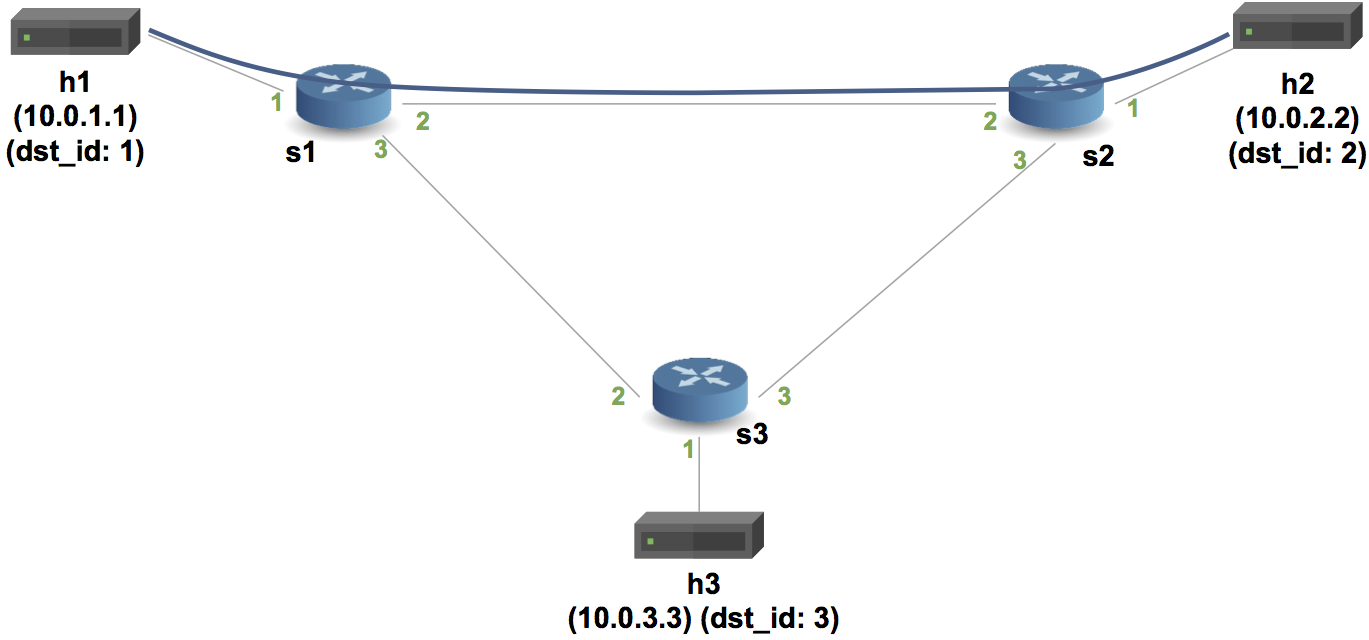
\includegraphics[width=\linewidth]{./img/test/8.png}
    \caption{Escenario a recrear.}
  \label{fig:yo}
\end{figure}
\newpage

Para cumplir el primer requerimiento se ha procedido de forma análoga al Test 1. Hemos extraído la cabecera de Ethernet, acto seguido hemos hecho un select en función del valor del EtherType, para parsearla cabecera Ipv4 o myTunnel.
\begin{figure}[!htb]
  \centering
    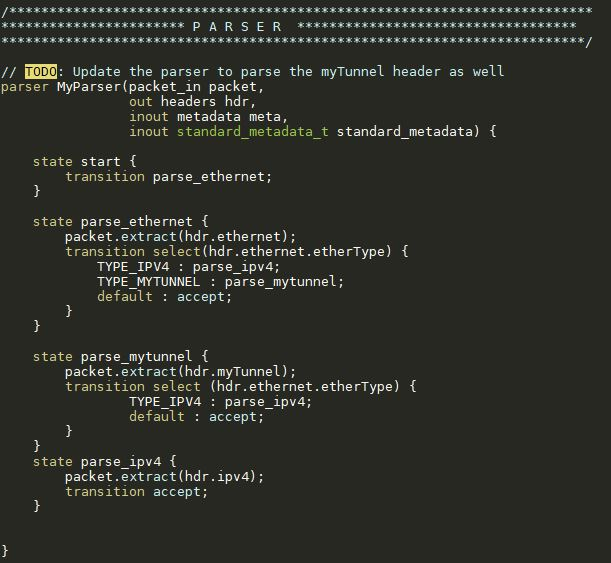
\includegraphics[width=0.7\linewidth]{./img/test/9.JPG}
    \caption{Parser actualizado.}
  \label{fig:yo}
\end{figure}

Hemos creado la nueva acción para hacer el forward hacia en puerto de salida dado por el plano de control. Esto lo especificamos indicándolo en los meta-datos asociados a ese paquete en el campo de egress port.
\begin{figure}[!htb]
  \centering
    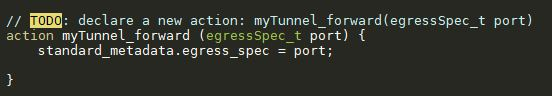
\includegraphics[width=0.7\linewidth]{./img/test/10.JPG}
    \caption{Nueva acción de forwarding.}
  \label{fig:yo}
\end{figure}
\newpage
\begin{figure}[!htb]
  \centering
    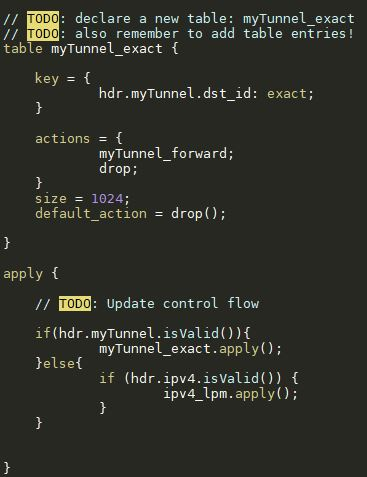
\includegraphics[width=0.5\linewidth]{./img/test/11.JPG}
    \caption{Nueva tabla de nuestro router.}
  \label{fig:yo}
\end{figure}
Para definir la nueva tabla hemos aplicado un criterio de búsqueda exacto, y que lo haga en función del dst\_id de la cabecera parseada. Si no hubiera ningún hit, por defecto se descarta el paquete. El campo  apply también ha sido actualizado para que primero se pase por la tabla de myTunnel\_exact en caso de que exista una cabecera valida de myTunnel, en caso contrario se sigu pasando por la tabla ipv4\_lpm.\newline
\newline
\begin{figure}[!htb]
  \centering
    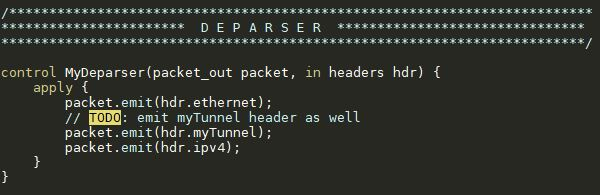
\includegraphics[width=0.8\linewidth]{./img/test/12.JPG}
    \caption{Deparser actualizado.}
  \label{fig:yo}
\end{figure}
\newline
En cuanto al Deparser únicamente se ha añadido la sentencia packet.emit(hdr.myTunnel). Esto hará que en caso de haber un paquete que contenga la cabecera myTunnel y que esta se validad, la serializará. En caso contrario omitirá esta sentencia. 
\newpage



